%\placelogofalse
\begin{frame}{UFL Applications}
\begin{columns}
\column{0.58\linewidth}
\centering
\begin{outline}
  \1 Write your equations in math-like notation
  \1 Get an efficient solver
  \1 General purpose
  \2 Cardiac modeling
  \2 Plasma Physics
  \2 Fracture Mechanics
  \2 Differentiable Physics
  \2 Parameter Estimation
  \2 Optimization
\end{outline}

\column{0.38\linewidth}
\begin{center}
\centering
%\shadowimage[width=2.5cm]{example_1.png}

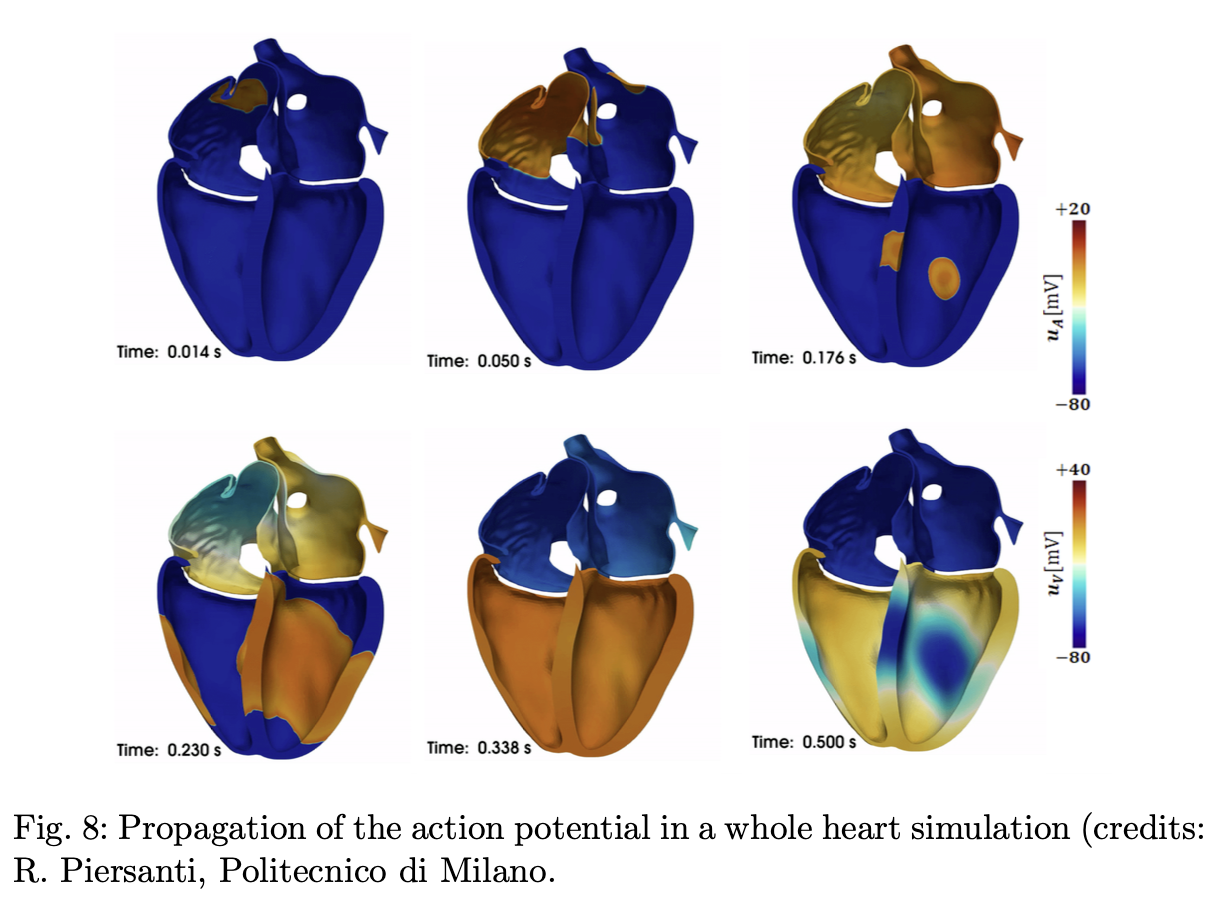
\includegraphics[width=4.5cm]{assets/cardiac.png}

\vspace{0.2cm}

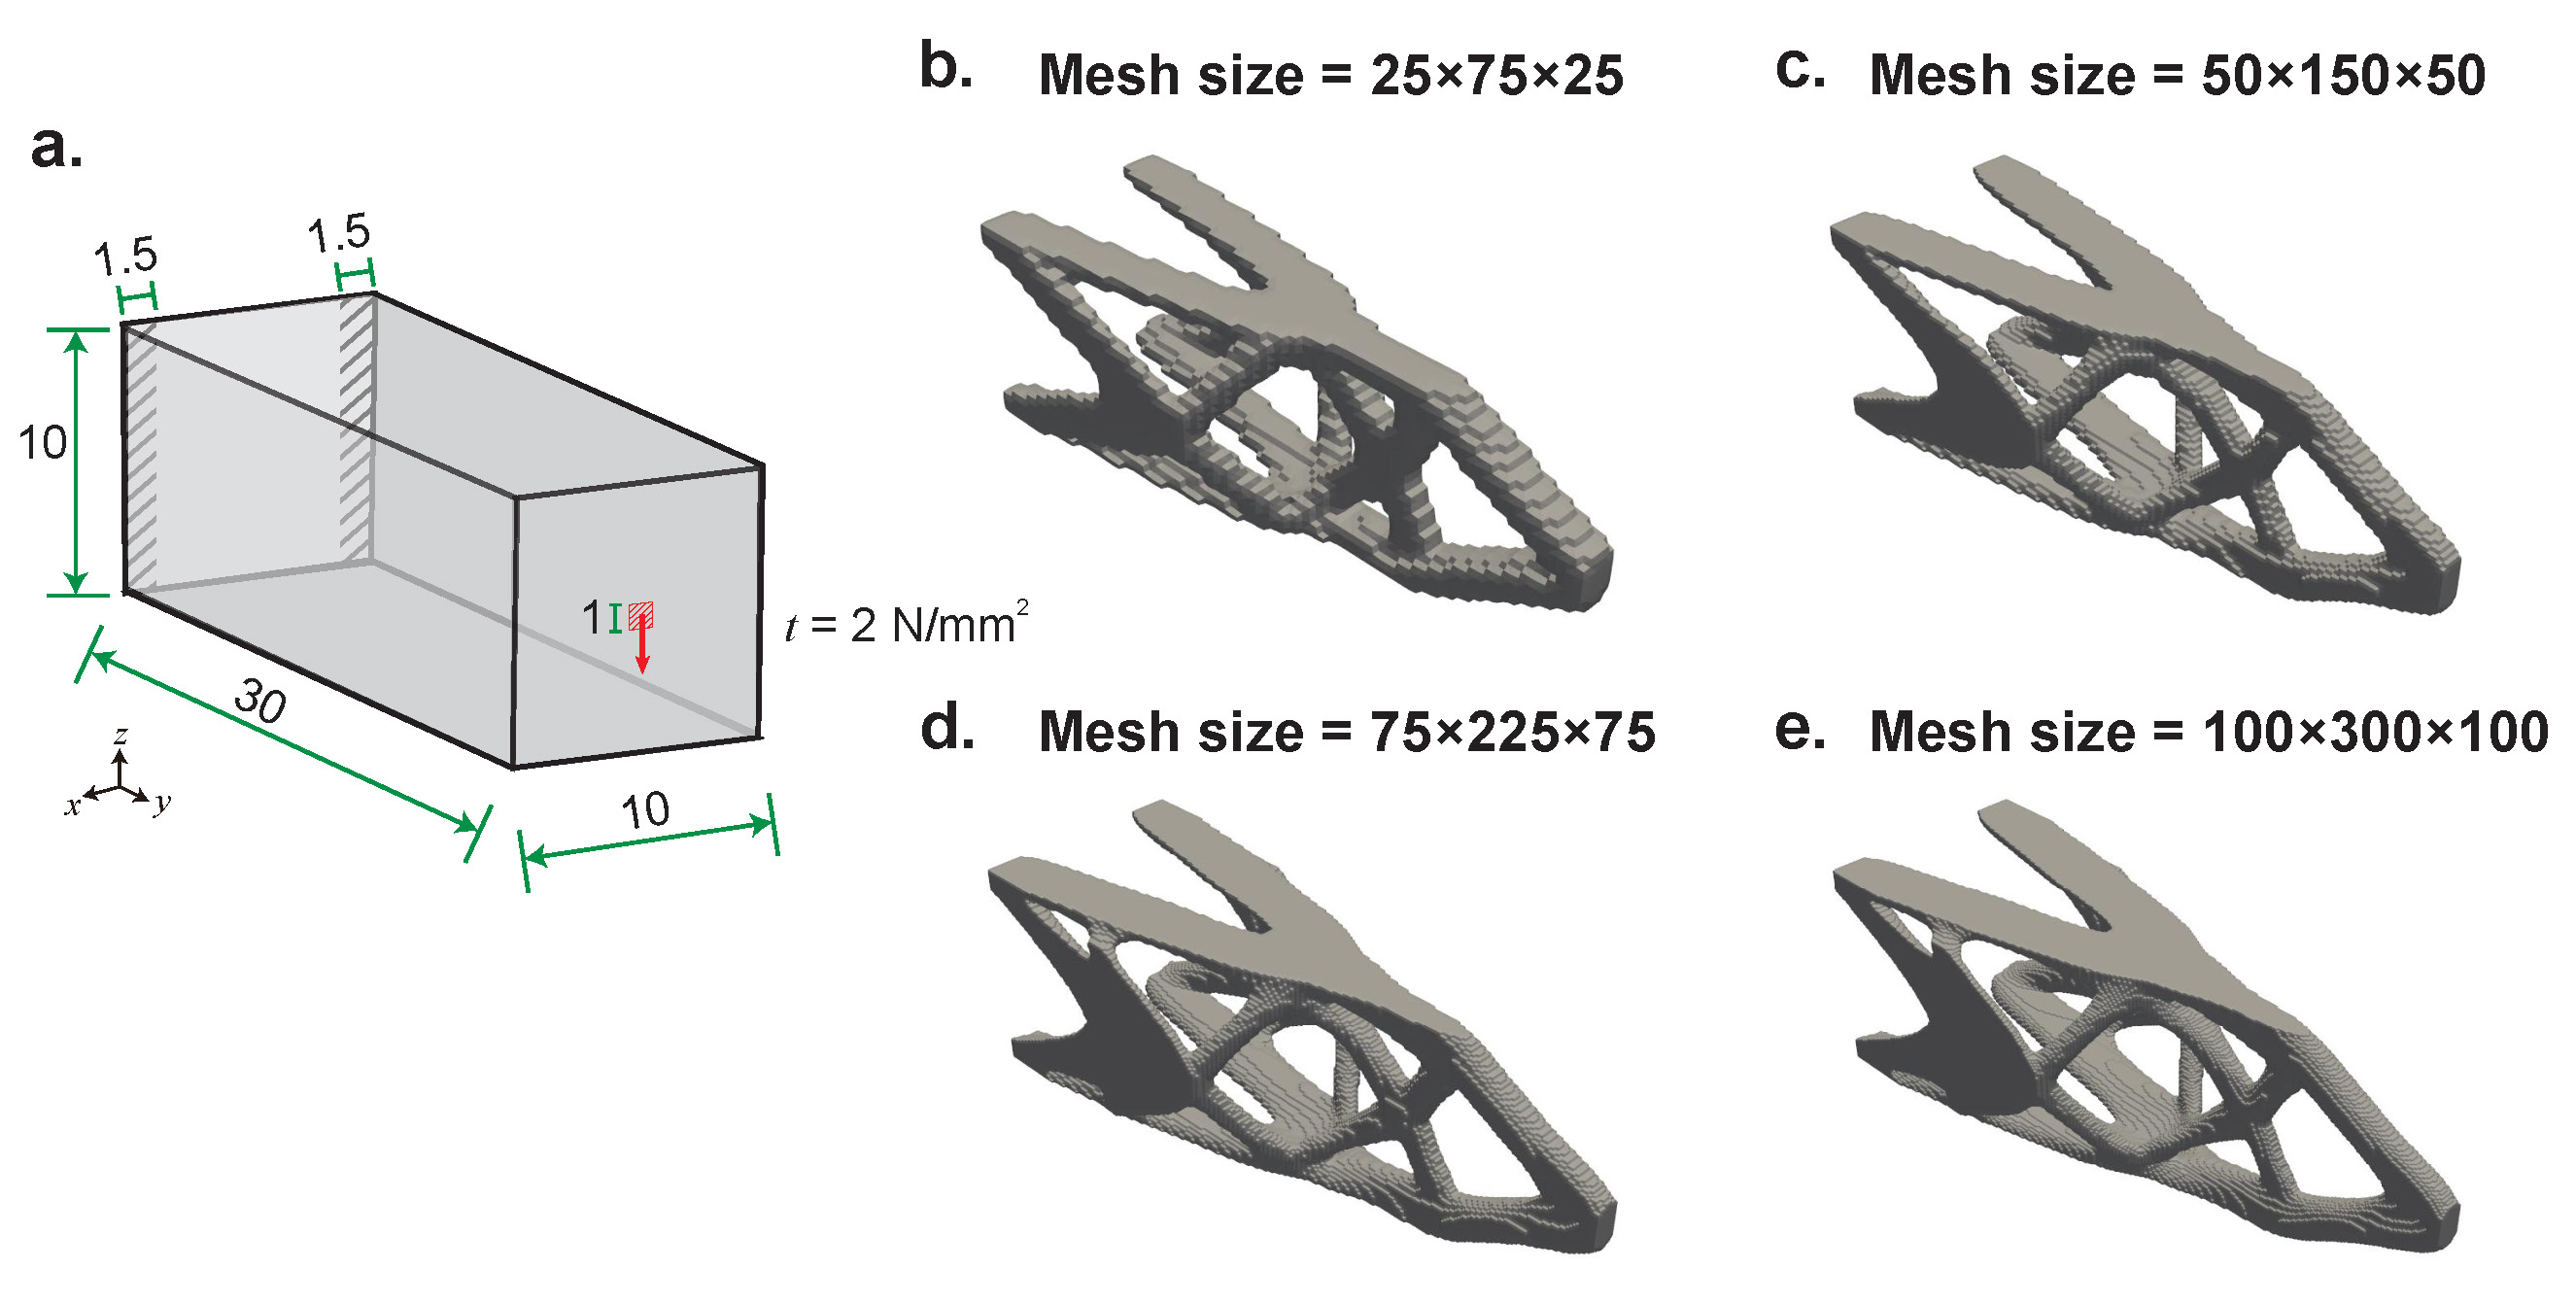
\includegraphics[width=4.5cm]{assets/beam_3d.jpg}


% [trim={left bottom right top},clip]
%
\includegraphics[width=8.5cm, page=3, trim={0 9cm 14cm 0cm},clip]{assets/vec_db_figs.pdf}
\end{center}
\end{columns}
\end{frame}
%\placelogotrue
